% 
% Annual Cognitive Science Conference
% Sample LaTeX Paper -- Proceedings Format
% 

% Original : Ashwin Ram (ashwin@cc.gatech.edu)       04/01/1994
% Modified : Johanna Moore (jmoore@cs.pitt.edu)      03/17/1995
% Modified : David Noelle (noelle@ucsd.edu)          03/15/1996
% Modified : Pat Langley (langley@cs.stanford.edu)   01/26/1997
% Latex2e corrections by Ramin Charles Nakisa        01/28/1997 
% Modified : Tina Eliassi-Rad (eliassi@cs.wisc.edu)  01/31/1998
% Modified : Trisha Yannuzzi (trisha@ircs.upenn.edu) 12/28/1999 (in process)
% Modified : Mary Ellen Foster (M.E.Foster@ed.ac.uk) 12/11/2000
% Modified : Ken Forbus                              01/23/2004
% Modified : Eli M. Silk (esilk@pitt.edu)            05/24/2005
% Modified : Niels Taatgen (taatgen@cmu.edu)         10/24/2006
% Modified : David Noelle (dnoelle@ucmerced.edu)     11/19/2014

%% Change "letterpaper" in the following line to "a4paper" if you must.

\documentclass[10pt,letterpaper]{article}

\usepackage{cogsci}
\usepackage{pslatex}
\usepackage{apacite}
\usepackage{graphicx}
%\usepackage{subcaption}
\usepackage{amssymb}
\usepackage{amsmath}
\usepackage{breqn}
\usepackage{url}
\usepackage{float}

\title{[Cute title]: The Pragmatics of Spatial Language}
 
%\author{{\large \bf Morton Ann Gernsbacher (MAG@Macc.Wisc.Edu)} \\
%  Department of Psychology, 1202 W. Johnson Street \\
%  Madison, WI 53706 USA
%  \AND {\large \bf Sharon J.~Derry (SDJ@Macc.Wisc.Edu)} \\
%  Department of Educational Psychology, 1025 W. Johnson Street \\
%  Madison, WI 53706 USA}

\author{
{\large \bf Author 1 (email@place.edu)} \\
  Department of Psychology, University of Gondor\\
  \And{\large \bf Author 2 (email@place.edu)} \\
  Department of Cognitive Science, University of Mordor \\
  \\
 \AND{\large \bf Author 3 (email@people.edu)} \\
  Department of Computer Science, University of Shire\\
}

\begin{document}
\maketitle

\begin{abstract}
People use spatial language

\textbf{Keywords:} 
Pragmatics, implicature, spatial language
\end{abstract}

\section{Introduction}

The spatial world is rich and complex, but the spatial language we use is often coarse and limited. For example, English---like many other languages---has a restricted and closed class of spatial prepositions~\cite{talmy83,talmy00,landau93} such as ``in,'' ``on,'' and ``near'' that describe a potentially infinite set of spatial relations. This raises a natural question: How do we make accurate inference in spatial situations when our spatial vocabulary is somewhat impoverished?

A plausible solution to this question is via pragmatic reasoning~\cite{}. By this view, listener would make inferences that go beyond the literal meaning of speaker's utterance by taking speaker's perspective in a given context. After all, inference is cheap and articulation is expensive~\cite{levinson00}, and we expect pragmatics to play a key role in enriching the core spatial vocabulary that can be limited under many different situations. 

To illustrate this idea, we describe a simple scenario that provides the basis of our study. Figure~\ref{illustration} shows the map of a small city with two quarters (i.e. represented by the red and blue rectangles respectively) and a plaza (i.e. represented by the dashed circle), where the plaza is located inside the red quarter. Suppose you were told that ``a gold lily grew in the red quarter.'' Where would you think the flower had grown on the map? There are two possiblilities. In the first case, a listener who takes the literal meaning of ``in'' would infer the lily to have grown anywhere within the red square. This follows from the fact that the core meaning of ``in'' would simply refer to locations within the enclosure of the red rectangle as bounded by its sides. However, a more sophisticated listener might instead reason as follows for a more precise spatial inference: ``If the lily had grown in the plaza, the speaker would have said that the lily grew in the plaza. However, given that she didn't say so, the lily must have grown within the red quarter but in areas excluding that plaza.'' Thus, this pragmatic listener would be able to make a more specific prediction than the literal listener about where the lily might have grown, even though the speaker's utterance is identical in both cases. In this respect, pragmatic reasoning helps the listener to locate things beyond the precision of what the meaning of ``in'' conventionally renders by combining perspective taking (i.e. playing the role of speaker) with one's knowledge of the spatial situation (i.e. the fact that the plaza is located inside the red square).

\begin{figure}[H]
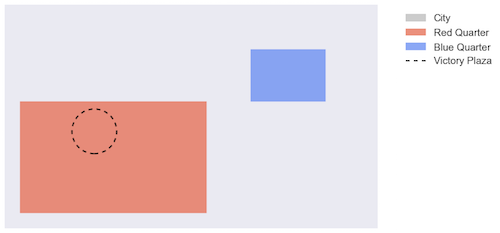
\includegraphics[scale=.5]{figures/cityA1.png}
\caption{Illustration of a simple spatial situation.}
\label{illustration}
\end{figure}

In this study, we explore the pragmatics of spatial language using probabilistic programs~\cite{}. MAYBE NOAH CAN SAY SOMETHING HERE? Previous work has discussed the role of pragmatics in spatial locative expressions~\cite{herskovits85,herskovits87}. However, to our knowledge, formal work in this domain is scarce. Moreover, recent computational studies have emphasized speaker's role in the pragmatic use of spatial language~\cite{carstensen14,golland10}, but not how listener makes pragmatic inference based on implicatures. We seek to bridge this gap with a formal model that makes quantitative predictions about listener's behavior as guided by spatial language and pragmatics. 

\section{Modeling spatial implicature}\label{mod}

Let's model it!

\section{Experiment}\label{sec:exps}

Let's test it with. 

\subsubsection{Participants} Here's who we asked. 

\subsubsection{Method.} This is what we asked them. 

\subsubsection{Results.} This is what they answered. 

\section{Comparison to model}

Hooray for implicature (p<0.05)

\section{Discussion}

Slack n such

\bibliographystyle{apacite}
\setlength{\bibleftmargin}{.125in}
\setlength{\bibindent}{-\bibleftmargin}
\bibliography{cogscibib}
\end{document}
